\section{Overview of graph summarization methods}
\label{sec:gc:methods}

There are many different ways to summarize a graph. However, akin to how a
correlation coefficient cannot sufficiently capture all aspects of dependency 
on its own, there is no single summarization method that can summarize 
every quality of a graph on its own. As such, this section discusses various 
graph summarization methods, the qualities that they measure, and their 
drawbacks. Furthermore, it is useful to normalize the returned 
summarization difference in order to understand the value scale properly, so a 
normalization method is proposed for each metric difference. 
In section~\ref{sec:gc:simulations}, we propose a method to select the most 
similar graph pair given a vector of differences where each difference 
corresponding to one of the six summarization methods listed below.

Most methods listed below are implemented in the \texttt{igraph} package in 
R~\cite{igraph}. As such, we do not implement most methods ourselves 
as we did in Chapter~\ref{ch:al}. The code for 
all methods may be found in Appendix~\ref{sec:appendicies:gc:engine}. It should 
be noted that there are various distance functions that may be used. 
Euclidean distance, L1, and L2 are currently implemented (code for the 
distance functions may also found in Appendix~\ref{sec:appendicies:gc:engine}). 

For all methods below, let $\hat{G}=(V,E)$ be some labeled graph.

\subsection{Centrality}
\label{sec:gc:methods:centrality}

The centrality of a graph $\hat{G}$ measures the importance of its 
nodes. Let $c$ be a vector of length $|V|$ where each element 
$c_i$ is the ``importance'' of node $i$. Then the centrality of $\hat{G}$ is 
given by~\cite{igraph}:
$$\mathcal{C} = \sum\limits^{|V|}_{i=1} \max_{\forall j \in \{1,...,|V|\}} 
c_j - c_i$$

\noindent The importance of each node may be measured by utilizing metrics such 
as~\cite{igraph}:

\tablespacing
\begin{itemize}
	\item \textbf{Degree:} 
	The degree of a node is the number of edges the node 
	is part of. In other words, it is the number of direct paths from the node 
	to all other nodes. The higher the degree, the more important the node 
	is.
	\item \textbf{Closeness:} 
	The closeness of a node is the average 
	shortest path length (the path which traverses the smallest number of 
	edges) between the node and all other nodes. The higher the closeness, 
	the closer the node is to all other nodes (in terms of path length), the 
	more important the node is.
	\item \textbf{Betweenness:} 
	The betweenness of a node is the number of 
	times the node is part of the shortest path between two other nodes. Direct 
	paths are excluded. The higher the betweenness, the more important the node 
	is as it provides a critical cost-saving link (path length) for the path 
	between many other nodes. 
\end{itemize}
\bodyspacing

The normalized centrality of a graph $\hat{G}$ may be computed as 	
$\frac{\text{Cen}(\hat{G})}{\max \text{Cen}(\hat{G})}$ where 
$\max \text{Cen}(\hat{G})$ is the 
maximum centrality that graph $\hat{G}$ may have (for whatever metric is 
specified). Taking the difference between two normalized scalars will also 
yield a normalized scalar.
Degree centrality is implemented in \texttt{centr\_degree}, 
closeness centrality is implemented in \texttt{centr\_clo}, and betweenness 
centrality is implemented in \texttt{centr\_betw} from the \texttt{igraph} 
package. By default, each function normalizes the returned centrality 
coefficient.

Now consider a graph whose edges are rotated as in 
Figure~\ref{fig:gc:drawbacks_rotation}; the centrality of the overall graph 
will not change as the edges are in the same relative positions, but the graph 
itself is clearly different. The computed centrality difference (with distance 
function L2 and for all centrality types) between the graphs pictured in 
Figure~\ref{fig:gc:drawbacks_rotation} is 0, which suggests they are exactly 
the same. This is due to the ``global'' nature of the centrality metric, which 
ignores the individual label of the nodes. Thus, when edges are rotated and 
nodes change, the graph ``looks'' exactly the same.
Should centrality be examined at node-level and not at a graph-level, 
this issue would be accounted for, though normalization is not as trivial. It 
is more difficult to efficiently parse node-level metrics 
especially in high dimensions, so this thesis does not detail or implement this 
metric.

\subsection{Assortativity}

Assortativity measures the level of resemblance among the connected nodes of a 
graph $\hat{G}$ based on vertex category labels. For graphs with uncategorized 
nodes (as in the examples of this chapter and the 
application in Chapter~\ref{ch:usage}), it is common to use $\text{deg}(V_i)-1$
as the category label for node $V_i$ instead~\cite{igraph}. 
For all edges $E_{i,j}$ that 
exist in $\hat{G}$, the degree of all associated nodes $V_i$ and $V_j$ are 
collected in two distinct vectors $v^1, v^2$. For instance, if $|V| = 4$ and 
$\hat{G}$ contained the set of edges $\{(1,2), (1,3), (2,4)\}$, then $v^1 = 
<2,2,2>$ and $v^2 = <2,1,1>$. Then the assortativity metric of a graph 
$\hat{G}$ is computed~\cite{newman2002}:
$$\mathcal{A} = \hat{\rho}^\text{Pear}(v^1,v^2)$$

\noindent where $\hat{\rho}^\text{Pear}$ is the Pearson 
correlation as defined in Section~\ref{sec:intro:correlation}. As such, 
the assortativity of $\hat{G}$ is summarized in a single value 
$-1 \leq \mathcal{A} \leq 1$ where the interpretation is the same as that of 
the Pearson correlation coefficient. For instance, $\mathcal{A}=1$ when nodes 
with high/low degrees in $\hat{G}$ are mostly connected to other nodes with 
high/low degrees in $\hat{G}$, respectively. In other words, if 
$\mathcal{A}$ is large, then connected vertices tend to have the same 
qualities, and when $\mathcal{A}$ is small, then connected vertices tend to 
have opposite qualities. Since assortativity involves a correlation 
computation, the result is already normalized. Again, taking the difference 
between two normalized scalars will also yield a normalized scalar.
Assortativity is called with the \texttt{assortativity\_degree} function from 
the \texttt{igraph} package.

Similarly, the assortativity difference metric is susceptible to rotated edges 
as shown in Figure~\ref{fig:gc:drawbacks_rotation}. Assortativity is another 
``global'' metric that measures the correlation among the degree of nodes but 
does not care about the exact nodes themselves. As such, the metric can be 
potentially misleading in situations where the actual nodes matter. In fact, 
the computed difference (with distance function L2) between the graphs in 
Figure~\ref{fig:gc:drawbacks_rotation} is 0.0032, which suggests the graphs are 
very similar when they are (visually) different.







\begin{figure}[htb]
	\begin{center}
		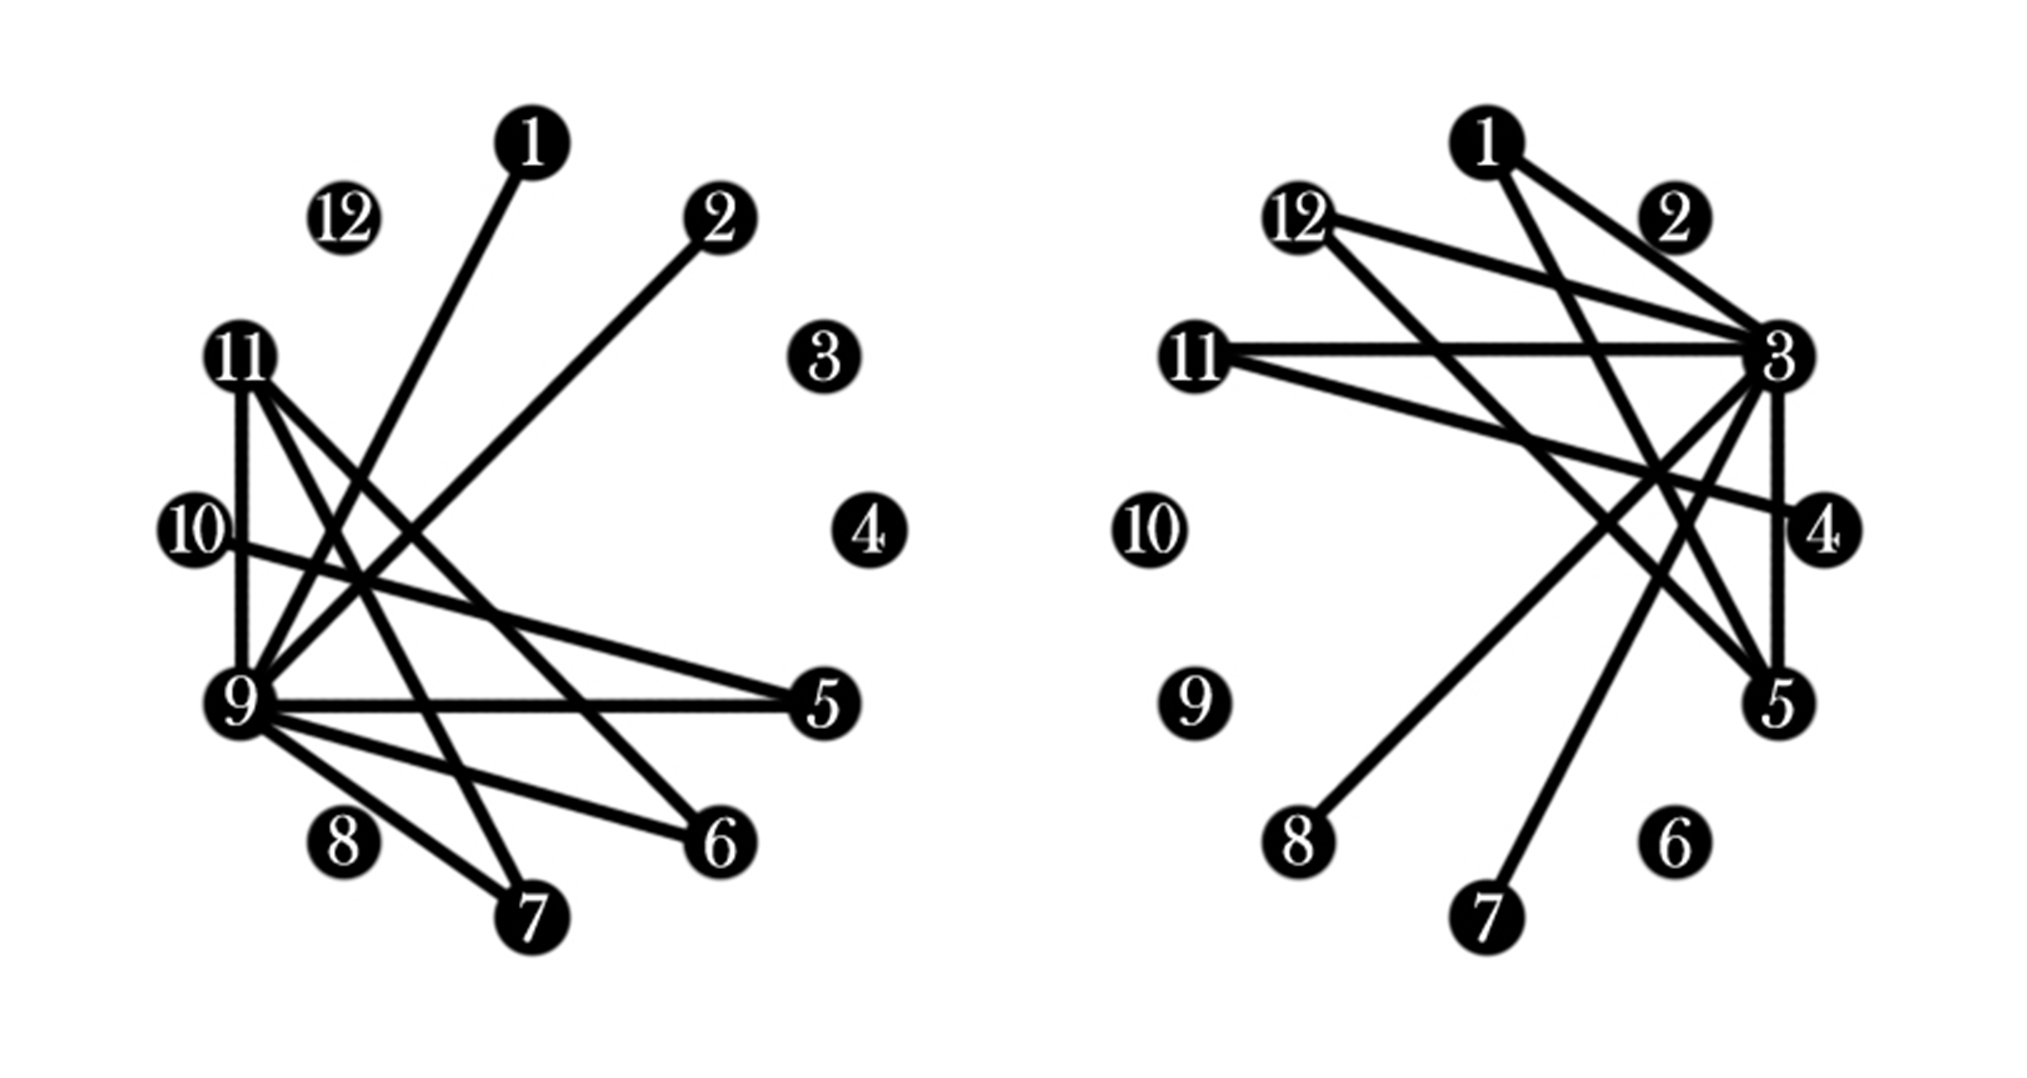
\includegraphics[width=1\linewidth]{ch-gc/figures/drawbacks_rotation}
		\caption[A graph pair with rotated edges.]{A graph pair with rotated 
			edges. These labeled graphs are clearly different from each other. 
			Graph summarization differences (L2 difference function): 
			
			\begin{tabular*}{.857 \textwidth}{ | c | c | c | }
				\hline
				Centrality (degree) & Centrality (closeness) & Centrality 
				(betweenness) \\
				\hline
				0 & 0 & 0 \\
				\hline
			\end{tabular*}
			\begin{tabular*}{0.984 \textwidth}{ | c | c | c | }
				\hline
				Community (random walk) & Community (infomap) & Community 
				(betweenness) \\
				\hline 
				0.9677 & 0.9677 & 0.9677 \\
				\hline
			\end{tabular*}
			\begin{tabular*}{0.947 \textwidth}{ | c | c | c | c | }
				\hline
				Assortativity & Distance matrix & Edge connectivity & Edge 
				density 
				histogram \\
				\hline
				0 & 0.3557 & 0 & 0 \\ 
				\hline
			\end{tabular*}
		}
		\label{fig:gc:drawbacks_rotation}
	\end{center}
\end{figure}





\subsection{Community}

The community of a graph $\hat{G}$ is given by $\mathcal{S}$, a set of its 
dense subgraphs. Subgraphs may be detected with any of the following 
algorithms~\cite{igraph}:

\tablespacing
\begin{itemize}
	\item \textbf{Random walks:} 
	By implementing a random walk within a graph 
	to determine the various subgraphs (or, in other words, to ``describe'' the 
	community), this procedure leverages the natural idea 
	that random walks within a graph will tend to stay in the same subgraph. 
	This occurs because a subgraph is often densely connected within itself but 
	sparsely connected to other subgraphs, so there is an increased probability 
	of proceeding via an edge that is within the same subgraph.
	This approach to building a community is called with the 
	\texttt{cluster\_walktrap} function from the \texttt{igraph} package.	
	
	\item \textbf{Infomap:} 
	An infomap utilizes random walks to build a 
	community by minimizing the expected length that it takes a random walk 
	to ``describe'' the community.
	This approach to building a community is called with the 
	\texttt{cluster\_infomap} function from the \texttt{igraph} package.
	
	\item \textbf{Betweenness:} 
	As described earlier, the betweenness of a node 
	is the number of times the node is part of the shortest path between two 
	other nodes (where direct paths are excluded). The algorithm sequentially 
	removes the node with the highest betweenness and places it on a tree, 
	recalculating betweenness of the existing graph every time a removal is 
	performed. This algorithm once again takes advantage of the natural idea 
	that subgraphs tend to be dense among themselves but with few edges 
	connecting them to other subgraphs. As such, edges which connect separate 
	subgraphs have high betweenness because all shortest paths from one 
	subgraph to another must pass through them. 
	This approach to building a community is called with the 
	\texttt{cluster\_edge\_betweenness} function from the \texttt{igraph} 
	package.
\end{itemize}
\bodyspacing

There is no way of normalizing $\mathcal{S}$ because it is not a numeric 
value. What is important to note, however, is that comparison among 
graphs $\hat{G^1}=(V^1,E^2)$ and $\hat{G^2}=(V^2,E^2)$ for the community graph 
difference computation (which \textit{does} return a numeric value)
must compare $\mathcal{S}^1$ and $\mathcal{S}^2$ with a method such as the 
Jaccard distance. Consider sets labeled $\mathcal{S}^1=(1,1,2,2,3,3)$ and 
$\mathcal{S}^2=(4,4,5,5,6,6)$. These are the exact same sets, but 
they are labeled with different values; thus, a traditional distance metric 
(e.g. Euclidean distance) would not capture the difference properly. 
The Jaccard distance compares the actual sets rather than their literal values, 
and it is already normalized between 0 and 1.
The Jaccard distance is obtained by subtracting the Jaccard similarity from 1. 
The Jaccard similarity is computed with the \texttt{cluster\_similarity} 
function in the \texttt{clusteval} package.

Where community has trouble is when a graph pair has many sparse clusters. 
Consider the simplified example found in Figure~\ref{fig:gc:drawbacks_comm}. 
While one graph has two physical clusters and the other has three, they are not 
all that visually different because only one edge has been removed. The 
community difference values are 0, 0.2727, and 0.2727 for random walk, infomap, 
and betweenness respectively.
Interestingly, the random walk community difference is 0; this is 
likely because it is a \textit{single random walk} which leaves more room for 
errors and may not fully explore the clustering structure especially if 
clusters are completely isolated as is the case in both graphs of the set 
illustrated in Figure~\ref{fig:gc:drawbacks_comm}. 
The values of 0.2727, on the other hand, are extremely significant when 
considering that the ``best case'' scenario where the split communities 
(6,7,8,9) and (10,11,12) from Figure~\ref{fig:gc:drawbacks_comm} (right) are 
\textit{perfectly recognized by the subgraph detection algorithm} yields a 
Jaccard difference of 0.3870968. 










\begin{figure}[htb]
	\begin{center}
		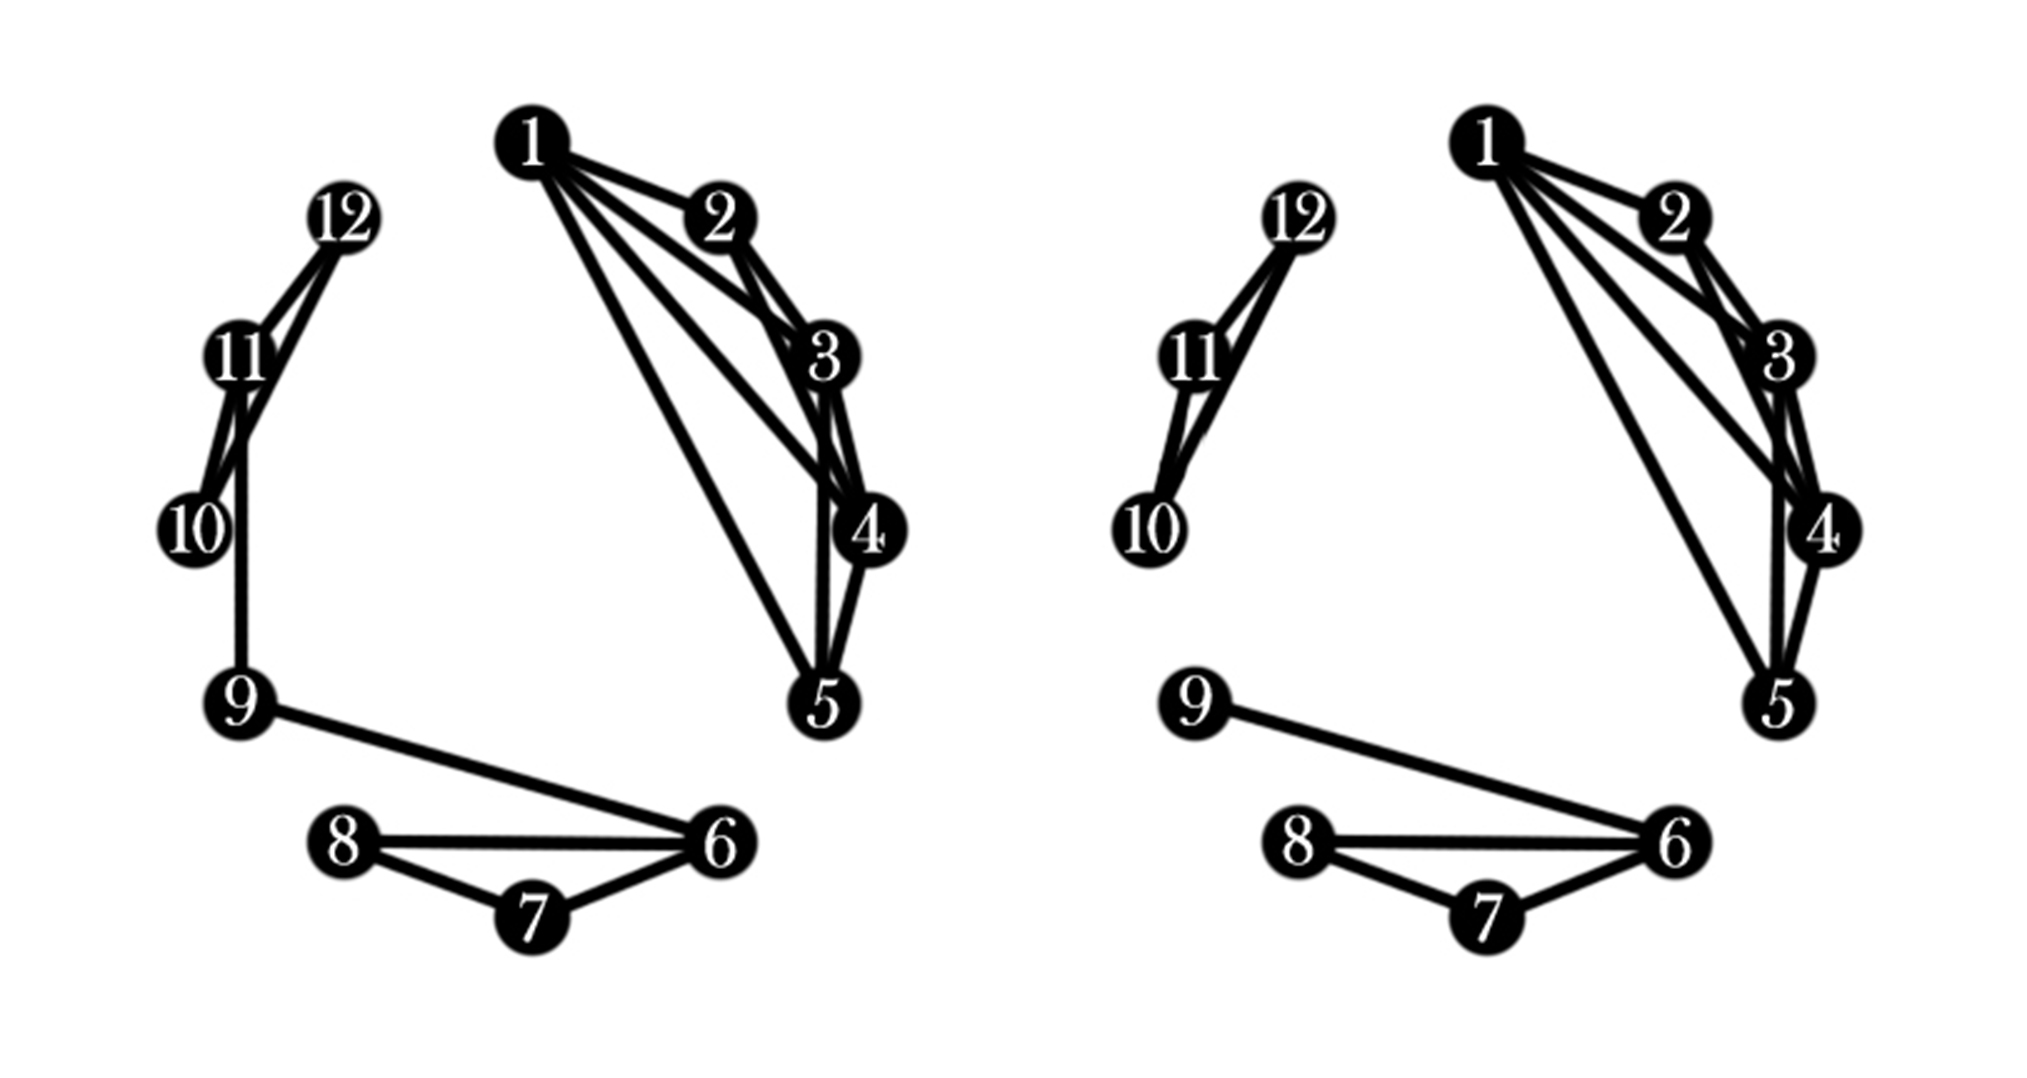
\includegraphics[width=1\linewidth]{ch-gc/figures/drawbacks_comm}
		\caption[A graph pair with two and three clusters, respectively.]{A 
			graph pair with two and three clusters, respectively. Only one edge 
			has been removed, so the graphs do not appear that extremely 
			different. Graph summarization differences (L2 difference function):
			
			\begin{tabular*}{.857 \textwidth}{ | c | c | c | }
				\hline
				Centrality (degree) & Centrality (closeness) & Centrality 
				(betweenness) \\
				\hline
				0.0002 & 0.0002 & 0.0102 \\
				\hline
			\end{tabular*}
			\begin{tabular*}{0.984 \textwidth}{ | c | c | c | }
				\hline
				Community (random walk) & Community (infomap) & Community 
				(betweenness) \\
				\hline 
				0 & 0.2727 & 0.2727 \\
				\hline
			\end{tabular*}
			\begin{tabular*}{0.947 \textwidth}{ | c | c | c | c | }
				\hline
				Assortativity & Distance matrix & Edge connectivity & Edge 
				density 
				histogram \\
				\hline
				0.0075 & 0.2233 & 0 & 0.0139 \\ 
				\hline
			\end{tabular*}
		}
		\label{fig:gc:drawbacks_comm}
	\end{center}
\end{figure}









\subsection{Distance matrix}

The distance matrix $M$ of a graph $\hat{G}$ is a square matrix that 
contains the shortest path length 
between all variable pairs; each element $M_{i,j}$ 
contains the shortest path distance between node $i$ to node $j$~\cite{igraph}. 
If no path exists, it is conventional to set the value to 
infinity~\cite{igraph}. However, since our 
purpose is to compare two matrices, setting a value of infinity doesn't 
make sense. Alternatively, the value may be set to zero since we define the 
shortest path distance in Section~\ref{sec:gc:methods:centrality} to be 
the path which traverses the smallest number of edges; thus, a 
\textit{direct path} between nodes has path length 1. Subsequently, the 
shortest path length can never be 0, which allows the 
existence of a ``non-existent path'' to be distinguished from the ``length of 
an existing path''. It is important to note that the matrix itself is repeated; 
the upper and lower triangles are the same. Furthermore, the diagonals are 0 by 
construction. Note that the matrix can be unfurled into a vector 
$m$ with the values of all $\binom{|V|}{2}$ unique pairs.
It is more difficult to normalize the distance matrix difference metric because 
it is hard to say what the upper bound on this difference is. For instance, one 
might think that the upper bound occurs when the distance matrix for one graph 
is of all 0's (i.e. an empty graph), and the distance matrix for the other 
graph is of all $|V|-1$ in the upper and lower triangles (the longest possible 
path length). However, it is actually impossible to construct a graph such that 
every node's \textit{shortest path} to all other nodes is exactly length 
$|V|-1$ (which is also the maximum possible degree).
Instead, it would be simplest to use the difference between the distance matrix 
of an empty graph and the distance matrix of a graph with a single Hamiltonian 
path (a path that visits each vertex exactly once) as the upper bound. This 
yields a bound that is actually slightly above 1 (i.e. the
difference is close to, but not exactly, the maximum possible distance matrix 
difference), but it is close enough for the purposes 
of interpretation. 
The distance matrix method is called with the \texttt{distances} function from 
the \texttt{igraph} package. \texttt{distances} returns infinity when a path 
doesn't exist, so the output is adjusted accordingly.

The distance-matrix is more granular. Because the metric relies on the shortest 
paths between all unique pairs of nodes, it is a node-level metric. As such, 
edge rotation is not 
a problem, but clustering becomes an issue when there are few clusters. 
Consider Figure~\ref{fig:gc:drawbacks_cluster}; the removal of edge (4,5) 
forces the shortest path between pairs with a node from each cluster to drop to 
0 and has a strong effect on the distance matrix distance since many pairs are 
now disconnected. 
The actual distance matrix difference for the graphs pictured in 
Figure~\ref{fig:gc:drawbacks_cluster} is 0.7708, which suggests that the graphs 
are very different when they are actually quite similar visually (only one edge 
has changed, so the mind perceives the same clustering structure). 
Although Figure~\ref{fig:gc:drawbacks_comm} is similar to 
Figure~\ref{fig:gc:drawbacks_cluster} in that both involve cluster 
manipulation, the larger number of clusters in 
Figure~\ref{fig:gc:drawbacks_comm} ensures that disconnecting two clusters will 
not change the distance matrix difference as much; less of the graph is 
interconnected, so fewer pairs will have a distance of 0. In fact, the distance 
matrix difference of Figure~\ref{fig:gc:drawbacks_comm} happens to be 0.2233, 
which is much lower than the distance matrix difference of 
Figure~\ref{fig:gc:drawbacks_cluster}. 









\begin{figure}[htb]
	\begin{center}
		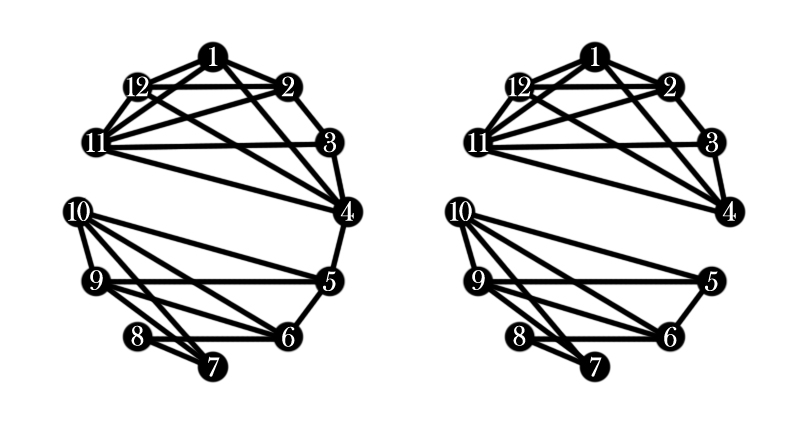
\includegraphics[width=1\linewidth]{ch-gc/figures/drawbacks_cluster}
		\caption[A graph pair with one and two clusters, respectively.]{A 
			graph pair with one and two clusters, respectively. Only one 
			edge has been removed, so the graphs do not appear that extremely 
			different. Graph summarization differences (L2 difference function):
			
			\begin{tabular*}{.857 \textwidth}{ | c | c | c | }
				\hline
				Centrality (degree) & Centrality (closeness) & Centrality 
				(betweenness) \\
				\hline
				0.0002 & 0.0899 & 0.1933 \\
				\hline
			\end{tabular*}
			\begin{tabular*}{0.984 \textwidth}{ | c | c | c | }
				\hline
				Community (random walk) & Community (infomap) & Community 
				(betweenness) \\
				\hline 
				0 & 0 & 0 \\
				\hline
			\end{tabular*}
			\begin{tabular*}{0.947 \textwidth}{ | c | c | c | c | }
				\hline
				Assortativity & Distance matrix & Edge connectivity & Edge 
				density 
				histogram \\
				\hline
				0.0032 & 0.7708 & 0.25 & 0.0139 \\ 
				\hline
			\end{tabular*}
		}
		\label{fig:gc:drawbacks_cluster}
	\end{center}
\end{figure}










\subsection{Edge connectivity}

The edge connectivity of a graph $\hat{G}$ is given by $\mathcal{E}$, the 
number of edges that need to be deleted in order to disconnect 
$\hat{G}$ such that there exists two nodes $V_i,V_j$ in $\hat{G}$ which do not 
have a path between them~\cite{igraph}.
%More specifically, it is the number of edges that need to be 
%deleted so that $\hat{G}$ is partitioned into $k$ distinct subgraphs and is
%no longer ``strongly'' connected. 
As the metric is upper bounded by the minimum 
degree of any node within a graph, the metric may be normalized by computing 
$\frac{\mathcal{E}}{\min\limits_{i \in \{1,...,|V|\}} \text{deg}(V_i)}$. Then, 
the difference normalization will naturally follow.
The edge connectivity of a graph is computed 
with the \texttt{edge\_connectivity} function from the \texttt{igraph} package. 

It is natural to see where this metric could fall through the cracks as it also 
``global'' and ignores the labels of each node. Consider 
a graph whose edges are rotated as in Figure~\ref{fig:gc:drawbacks_rotation}; 
the number of edges needed to disconnect the graph won't change as the edges 
are in the same relative positions, but the graph itself is clearly different. 
In fact, the computed edge connectivity difference (with distance function L2) 
between the graphs pictured in Figure~\ref{fig:gc:drawbacks_rotation} is 0, 
which suggests they are the exact same.

\subsection{Edge density histogram}

The edge density histogram is not implemented in the \texttt{igraph} package; 
it is a simple summarization metric which we have derived from the notion of a 
standard/traditional histogram. 
This metric captures the number of nodes in a graph $\hat{G}$ that have a 
specified number of degrees. Naturally, a larger number of high-degree nodes 
signals that $\hat{G}$ is dense, and a larger number of low-degree nodes 
signals that $\hat{G}$ is sparse. For 
$\hat{G}$, the edge density is summarized in a 
vector $v$ of length $b$, the number of desired ``bins'' 
(e.g. bin 1 is $1-5$ degrees, bin 2 is $6-10$ degrees, etc.). Then the value 
$v_i$ is the number of nodes which correspond to bin $i$. This 
metric may be normalized by computing $\frac{v_i}{|V|}$ for 
all $i \in \{1,...,b\}$ since there are a total of $|V|$ nodes; thus, each bin 
is upper bounded by $|V|$. Normalizing the graph-specific metric $v$ then
allows the difference computation to be normalized. 

The edge density histogram difference metric is also susceptible to rotated 
edges as illustrated in Figure~\ref{fig:gc:drawbacks_rotation} because it 
aggregates nodes into bins, which discards the labels of each individual node; 
the number of high-degree and low-degree nodes 
will not change even if the edges are rotated, but the graph is still clearly 
different. In fact, the computed edge density histogram difference (with 
distance function L2) between the exact graphs in 
Figure~\ref{fig:gc:drawbacks_rotation} is 0, which suggests that the graphs are 
exactly the same.